\section{Research in logging practices}
\label{section-research-in-logging-practices}
Portions of the contents of this case study have been published in a jointly authored paper published at MOBILESoft 2021~\citep{harty2021_logging_practices_with_mobile_analytics}.

\begin{figure}
    \centering
    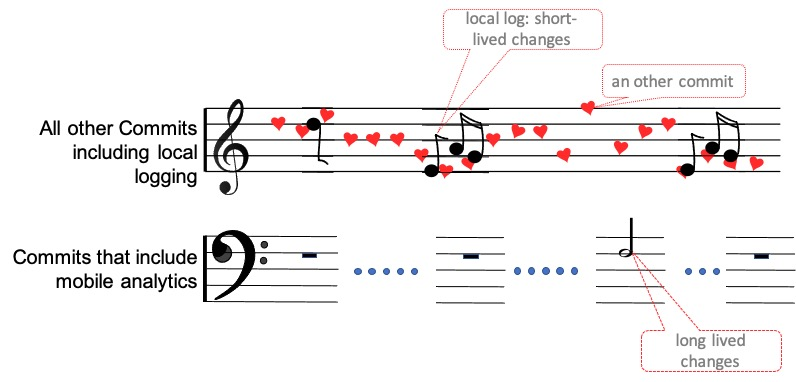
\includegraphics[width=15cm]{images/mobile-analytics-logging/musical-illustration.jpg}
    \caption{Musical representation of commits for local and mobile analytics logging}
    \label{fig:mobile_analytics_logging_musical_illustration}
\end{figure}

This case study investigates commits to various software repositories to determine their composition and characteristics of the frequency of those related to mobile analytics and the contents of the mobile analytics messages implemented in those commits. 

Commits to repositories may be hard to visualise; there is at least one software project that represents commits both visually and through sound, namely \href{https://github.com/debugger22/github-audio}{GitHub Audio} and available online~\url{https://github.audio/}~\footnote{Inspired by \href{http://listen.hatnote.com/\#}{Listen to Wikipedia} with the associated software project~\url{https://github.com/hatnote/listen-to-wikipedia}.} which does so. The patterns of commits this case study detected inspired a way to represent commits, their contents, and the longevity of their contents through music. Figure~\ref{fig:mobile_analytics_logging_musical_illustration} where each commit is represented as a heartbeat. Some include changes to local logging, some include changes to mobile analytics logging and these are represented by musical notes. Commits provide the tempo, the length of the note represented the length a particular change lives for where shorter notes represent short-lived changes, and longer notes represent long-lived changes. 

% The organ music score in https://music.stackexchange.com/questions/24426/what-does-grt-and-sw-mean-in-this-organ-score might be a good basis to develop my musical analogy. 

\subsection*{Rationale}
%\marian{Need to connect this case study with the thesis: what was the goal and show the key contributions. Rationale for this case study. which gave me the chance to look at .... Rationale for the intervention.}

This case study investigates and illustrates how developers have chosen to use mobile analytics to effectively provide remote logging from the field when their application is being used. The case study presents empirical research into characteristics of mobile analytics logging including the density of logging code, the frequency of updates to this code, and also what is being logged. Logging is an endemic practice in software engineering and the realisation that developers have chosen to use mobile analytics effectively for remote logging is relevant in terms of its use for measuring and potentially improving the reliability of their apps.

This case study gave me the chance to look at the historical practices of hundreds of developers of actively maintained Android apps. The goal was to increase understanding of what these developers have used the most popular and prevalent mobile analytics service (Firebase Analytics) for. It also presented an excellent opportunity for international collaboration with a mix of fledgling and highly experienced researchers in areas related to my research.

\textbf{Still TBD} how to weave in, and integrate, the earlier work Joe and I did to analyse local logging and the software we created to help analyse log messages. It was a precursor to the collaborative research and certainly helped inform my thinking and aspects of my collaboration with the rest of the authors, first at the Shonan, and then subsequently in the joint research that led to the MOBILESoft 2021 paper. In my view the work with Joe on log analysis aligns with the case study however none of us actually applied that work to the collaborative case study discussed in this section.

\par\noindent\rule{\textwidth}{0.4pt}

\subsection*{Contributions of this case study}
\begin{itemize}
    \item Insights into the footprint and overhead of what developers of 57 Android apps actively log, together with an understanding that developers of 50 more Android apps chose to simply integrate Firebase into their app and [presumably] rely on the default information Firebase provides them.
    \item An example of collaborative research I helped lead in an area related to my PhD.
    \item Identifying differences between internal and external logs/logging.
    \item A connection established between logging and mobile analytics.
    \item TBC the intersection between using mobile analytics \textit{and} crash reporting.
\end{itemize}


\setminted{fontsize=\small,baselinestretch=1}

\subsection*{Evidence}
  \begin{minted}[
    gobble=4,
    frame=single,
    fontsize=\tiny,
    breaklines=true
  ]{yaml}
    evidence available :
      public reproduction package : \url{https://github.com/mobileanalyticslogs/mobileanalyticslogging}
      local private reproduction : ~/sandbox/apmtracker and~\url{https://github.com/julianharty/research-in-logging-practices}
      co-written-paper : MOBILESoft 2021
      joedocs : various notes.
        \url{https://joedocs.com/julianharty/site/apm-logging-research}
      zoom : various meeting recordings.
      overleaf: drafts and the final paper for MOBILESoft 2021
    evidence-needed : 
      An assessment of which of the 107 projects also incorporate crash analytics.
      Review Luca's list of 8K verified Android apps on GitHub.
      Are any of the 107 apps on f-droid? How many are in the 8K verified Android apps from Luca Pascarella et al.?
  \end{minted}  

\subsection*{ad-hoc, interim, notes}
Notes from Skype call on 14 May 2021 for this case study in particular
\begin{enumerate}
    \item  Clearly separate temporary content from content intended to remain in the thesis.
    \item  Across a collection of apps and their characteristics
    \item  Limit the stuff off message. \textit{The message is to always connect Reliability, Mobile Analytics, and Software Engineering.}
    \item  Explain briefly that F-Droid is an app store that has these characteristics... 
    \item  Check the intersection between the 57 apps and those on F-Droid.
    \item  Commits provide the tempo - helps understand the illustration, the sonification, vs. does the audio help the developers improve their code.
    \item  It's OK to self-plagiarise provided I make this clear to the reader
\end{enumerate}


\subsection{Introduction}
\emph{(Highlight key features of case, similarities and differences w.r.t. other cases);}

This case study provides an additional perspective: that of investigating what various opensource Android developers have used Firebase Analytics for in their Android apps. It complements the development team case studies (where I worked with and/or interviewed the developers) by studying the contents and history of source code of 107 projects. It mines software repositories hosted on~\href{https://github.com/}{GitHub} and compares the use of the foremost mobile analytics SDK (Google's Firebase Analytics) for logging compared to the use of local logging.

Where these apps are in Google Play the developers would already have access to Google Play Console and Android Vitals, yet they have chosen to incorporate an additional analytics library into their app's codebase to log various details. 

Similarities to other case studies include: the projects are for live, actively maintained, Android projects and apps. Mobile Analytics is at the core of the case study. It investigates the use of mobile analytics by the development teams. The research has been collaborative in nature and aims to lead to further research.

We had two primary research questions for this case study:
\begin{enumerate}
    \item What are the characteristics of logging practices with mobile analytics?
    \item What do developers log in mobile analytics?
\end{enumerate}


\subsection{Context}
\emph{(Product/Project overview, Developer characteristics, tools, methods, key challenges for product/project);}

In this section, we present our case study and the results through answering our two research questions.

\noindent \textbf{Subjects.} Our study is based on analyzing 25,611 Java projects used in prior research of logging utilities practices~\cite{boyuanlogutility}. In particular, all the Java projects are obtained from the GHTorrent~\cite{10.5555/2664446.2664449} MySQL dump  (last updated on 2019-06-01). Duplicate (\textit{e.g.} forks and clones) projects were removed as were inactive projects. In order to identify the projects that use Firebase Analytics, we further filtered the projects by searching keyword ``FirebaseAnalytics'' in each project's source code and collected 107 projects. For each of the 107 projects we manually examined whether customised APIs are used by developers for mobile analytics logging. We found 50 of them only collect the default automated metrics generated by Firebase without proactively logging any information. Therefore, our study focuses on the remaining 57 projects where developers intentionally leverage the logging features in Firebase to collect information for their software.

\noindent \textbf{Identifying logging statements.} Initially we followed the same practice as prior research where logging statements are identified based on the Abstract Syntax Tree (AST) and the particular pattern of method invocation of each logging library~\cite{yizengemse,chen2017characterizing}. 
%
However, after manually examining the logging statements, we found \emph{developers often wrap the Firebase APIs in a custom logging class}. In particular, logging using the Firebase API is rather complex where multiple method invocations are often needed to 
log once. Therefore, developers rarely directly call the Firebase APIs to log. Instead, they create wrapper class that provides utility methods that log using the Firebase API.
% This is also hard to decipher.
We manually identified these wrapper classes and their utility methods. These methods were used as keywords to automatically identify the logging statements in their respective project.
%
Specifically, we leveraged srcML to convert source code files to XML files. (Kotlin source files were first renamed from \texttt{*.kt} to \texttt{*.java} which was enough to process them). We then extracted all the invocation calls by using XPath. Then, for each project we used regular expressions to check whether the caller names matched with the corresponding class names we found.


The project was initiated in December 2019 during various breakout sessions I participated in at Shonan Workshop 152~\citep{nii_shonan_workshop_152} where we, a group of researchers, agreed we would like to learn more about mobile analytics being used for logging by mobile apps. The initial group comprised of three late stage PhD students~\footnote{Two of these successfully defended their thesis during this case study.} and two associate professors. We were subsequently joined by an additional early stage PhD candidate who led the initial searches for suitable projects and who also wrote the source code and scripts used to perform the core analysis of these projects.

As one of the professors (\href{https://users.encs.concordia.ca/~shang/}{Weiyi Shang}) had extensive, recent, and relevant experience of two key and related aspects, namely 1) analysis of local logging practices in opensource Android apps~\citep{zeng2019studying_logging_practices_fdroid} and 2) in using the srcML analysis tool we used these to bootstrap our research. Similarly, the GHTorrent offline repository of GitHub projects~\citep{gousios2012_ghtorrent_githubs_data_from_a_firehose} was chosen for the initial selection and filtering of projects based on his recommendation and prior research experience. 


\subsubsection{Methods} 
%GHTorrent records the information of all the projects on GitHub. In the first step, we downloaded the most recent GHTorrent SQL dump and ruled out the projects (projects not in java or kotlin) we didn't need. In the second step, we further filtered these projects with FirebaseAnalytics. The first step was done by a previous master student in our lab, I started my work from the second step.  The GitHub HTTP queries are mainly used for further filtering the projects, the GraphSQL queries are mainly for getting the author information and the commit information etc. so that we can email the authors (we finally decided not to do the survey part so the information is not used). 

\textbf{Identify the projects to analyse}
The first pass was to identify Android apps on F-Droid~\citep{fdroidwebsite} that included Firebase Analytics. F-Droid is a small, alternative to Google Play for Android apps where the apps and the app store are all fully opensourced. There are currently just over 4,000 apps in May 2021~\footnote{Based on summing up the package counts for all the categories~\url{https://f-droid.org/en/packages/}.} % {Connectivity:213,Development:158,Games:378,Graphics:64,Internet:553,Money:109,Multimedia:432,Navigation:203,Phone \& SMS:91,Reading:187,Science \& Education:267,Security:179,Sports \& Health:136,System:545,Theming:166,Time:181,Writing:207} 
% See also https://en.wikipedia.org/wiki/F-Droid for various analysis of f-droid, at the time of writing it was several months out of date.
so it's a miniature app store, yet one that's used relatively frequently by researchers owing to the availability of the source code and visibility into the system and service compared to the Google and Apple app stores.

Only 7 were found to incorporate Firebase Analytics in the F-Droid source projects. We therefore decided to analyse public projects hosted on GitHub which hosts many more Android apps. (Counts vary, ~\citep{geiger2018_a_graph_based_dataset_of_commit_history_of_realworld_android_apps}, identified 8,431 actively maintained, live opensource Android apps matched on Google Play of a far larger set of unique Android apps identified by their package name.)

The most recent GHTorrent SQL dump that was available at the time, from \nth{1} June 2019~\footnote{The dump is available from \url{http://ghtorrent-downloads.ewi.tudelft.nl/mysql/mysql-2019-06-01.tar.gz} it's 102973 MB (source~\url{https://ghtorrent.org/downloads.html}) so best to only download when needed and practical to do so!}. This was filtered in two stages, first to exclude projects not in Java or Kotlin which resulted in 25,611 matches, and then those were filtered to select those that included FirebaseAnalytics (a compound word to match the relevant SDK in the source code) \textit{i.e.} for Firebase Analytics.

\textbf{Selecting active, real-world, apps}
GitHub.com contains a vast range of projects and the nature of git where forks of projects are encouraged and trivial to do meant we needed to filter out duplicates, toy, and inactive projects. Various signals were used to perform the filtering including the number of project stars, the volume and recency of commits, etc. GitHub HTTP queries were mainly used for further filtering the projects.

We also ran ad-hoc queries by searching for the keyword firebaseanalytics directly on GitHub for edification and to help the various authors participate and for sanity checks.
%
An example of the query is \url{https://github.com/search?q=\%22implementation+\%27com.google.firebase\%3Afirebase-analytics\%27\%22&type=Code}. These match a pattern used in \texttt{app/build.gradle} a standard file in virtually all Android projects. Listing~\ref{listing:trashout_ancient_firebaseanalytics_version} provides an example of one of the search results. A quick indication this project is no longer actively maintained is the version number at the end of the line of code, version 15.0.1 of Firebase Analytics was current in Spring of 2018 (as confirmed by the release history for Firebase: \url{https://firebase.google.com/support/release-notes/android#version_1502})~\footnote{Oddly this lists release 15.0.0 and 15.0.2 and does not have an entry for 15.0.1, yet 15.0.1 is found in examples online.}.

\begin{listing}
\begin{minted}[
    gobble=4,
    frame=single,
    fontsize=\tiny,
    breaklines=true
  ]{groovy}
      implementation 'com.google.firebase:firebase-analytics:15.0.1'
\end{minted}
\caption{Source~\href{https://github.com/TrashOut/Android/blob/e897c1c05629f3f5da23516fdfbd24870f773166/app/build.gradle\#L88}{Line 88 of app/build.gradle for TrashOut Android}}
\label{listing:trashout_ancient_firebaseanalytics_version}
\end{listing}
%%%% Note groovy is the language code to use for gradle, see https://pygments.org/docs/lexers/

\textbf{Identify the logging statements}

\begin{listing}
\begin{minted}[
    gobble=2,
    frame=single,
    fontsize=\tiny,
    breaklines=true
  ]{bash}
  % Sanity check of commits for the muzei Android app for messages that mention adding or revising analytics
  git log --oneline | grep -i analytics | grep -v Up | grep -v Merge | grep -v Disable | grep -v Convert | wc -l
\end{minted}
\caption{Bash command as a sanity check for commits mentioning analytics in the muzei Android repo}
\label{listing:sanity_check_muzei_android_commits}
\end{listing}


\textbf{Identify potential contributors to survey}
We performed preliminary analysis to identify the potential candidates for a survey. These include the person who made the first, second, and last commits. The script~\href{https://github.com/mobileanalyticslogs/mobileanalyticslogging/blob/76569d59f0ea6f49f9549433d24ae59dda7fedfd/util/repo\_info\_crawler.py}{util/repo\_info\_crawler.py} also identified the top three contributors to each of the repositories. 

GraphQL queries were mainly used that queried GitHub's GraphQL API~\footnote{\url{https://docs.github.com/en/graphql}} to obtain the author and the commit information \textit{etc.}. 

From an ethics perspective all these details are publicly and freely available \footnote{For example, the contributors for the OneBusAway Android app are available online at~\href{https://github.com/OneBusAway/onebusaway-android/graphs/contributors}{Contribotors to OneBusAway/onebusaway-android}.} and the people involved choose how much personal information to provide and can use pseudonyms, ~\emph{etc.}.

Note: We decided not to do the survey so the information was not used.


\textbf{Establish and maintain coherence across the team}
As a disparate group of individuals, from different cultures, various mother tongues, and working across multiple timezones (from Hong Kong to Quebec) there were multiple opportunities for confusion, misunderstandings, and miscommunication. As a group we therefore focused on establishing and maintaining coherence by having each person work with at least two others, through actively taking and sharing notes, and so on. Furthermore we established a common codebook with total agreement on the contents and the assignment of categories to each of the log lines in the `training set' used to calibrate us as a team and as a coherent group of researchers.  

\textbf{Establish the codebook}


\textbf{Apply the codebook on a larger, representative, sample}


\textbf{Key challenges} included finding suitable projects on f-droid, identifying suitable projects on GitHub, agreeing on the classifications, \href{subsection_srcml_working_with_kotlin_files}{working with Kotlin source files}, and the collaboration in general given the range of locations and timezones of the authors. 

\textbf{Methods for effective collaboration}
As a codicil to the methods section, here is a brief overview of the methods used to collaborate as researchers. 

We used a private GitHub repo for the data analysis and source code until the first paper was written. Overleaf was used as our collaborative editor for academic writing and subsequent publications. In addition two online services were used for written work: 1) google docs for ad-hoc documents and spreadsheets, and 2) \href{https://joedocs.com/}{JoeDocs}~\footnote{JoeDocs was co-created and is subsequently maintained by a friend, collaborator, and colleague - Joseph Reeve. JoeDocs provided a practical alternative to Google Docs, especially during the first lockdown for COVID-19 where various online services were struggling to cope.}. 

A series of meetings used Zoom video calls and many of these calls were recorded with the full agreement of the group so we could review to meetings afterwards, for instance if anyone missed a meeting. Of course, emails were also endemic. I made notes for many of the meetings and these are freely available for our group of researchers.

\subsubsection{Working with Kotlin source files}
\label{subsection_srcml_working_with_kotlin_files}

\begin{listing}
\begin{minted}[
    gobble=2,
    frame=single,
    fontsize=\tiny,
    breaklines=true
  ]{bash}
  # Download and install srcML from their project’s website

  srcml -V
  # 1.0.0 etc.

  srcml --show-language ./main/src/main/java/com/google/android/apps/muzei/MuzeiActivity.kt
  # no visible output

  ln -s  ./main/src/main/java/com/google/android/apps/muzei/MuzeiActivity.kt MuzeiActivity.java

  srcml --show-language MuzeiActivity.java#Java
  srcml MuzeiActivity.java -o MuzeiActivity.xml
  vim MuzeiActivity.*
\end{minted}
\caption{Bash commands to show how srcml can be coerced into analysing Kotlin files}
\label{listing:bash_example_srcml_does_kotlin}
\end{listing}

One of the challenges we encountered was in how to analyse source code written in Kotlin~\footnote{Kotlin is increasingly popular both for new Android apps and many developers are migrating code from Java to Kotlin in existing apps. 
%
Up to date estimates of the growth of Kotlin are available from AppBrain~\href{https://www.appbrain.com/stats/libraries/details/kotlin/kotlin}{Kotlin - Android SDK statistics | AppBrain}, for example.}. 
The software tool we used for this research, \href{https://www.srcml.org/}{srcML}, did not support Kotlin directly at the time of the case study, it only supported C, C++, Java and C\#. Our solution was crude yet appeared to be adequate for the purposes of our research; we created symbolic links for each Kotlin source file where the link has a \texttt{.java} extension. Listing~\ref{listing:bash_example_srcml_does_kotlin} illustrates the approach. We checked the XML files that srcML generated for these files together with the results of the regular expression matches to confirm this approach was sufficient~\footnote{Details about srcML including the XML it generates are available on the project's \href{https://www.srcml.org/about.html}{About} page}.

\subsection{Findings and Results}
\textit{(Describe what you did with analytics in the context of the case);} 



\begin{figure}[htbp!]
\centering
\begin{minipage}{.5\textwidth}
  \centering
  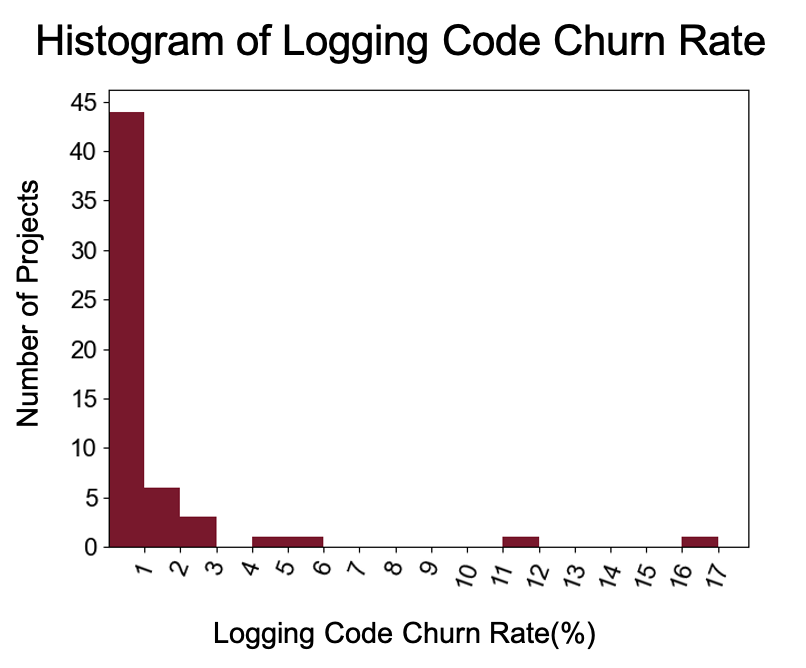
\includegraphics[width=.8\linewidth]{images/mobile-analytics-logging/logging-churn-rate.png}
  \captionof*{figure}{Churn}
  \label{fig:logging-churn-rate}
\end{minipage}%
\begin{minipage}{.5\textwidth}
  \centering
  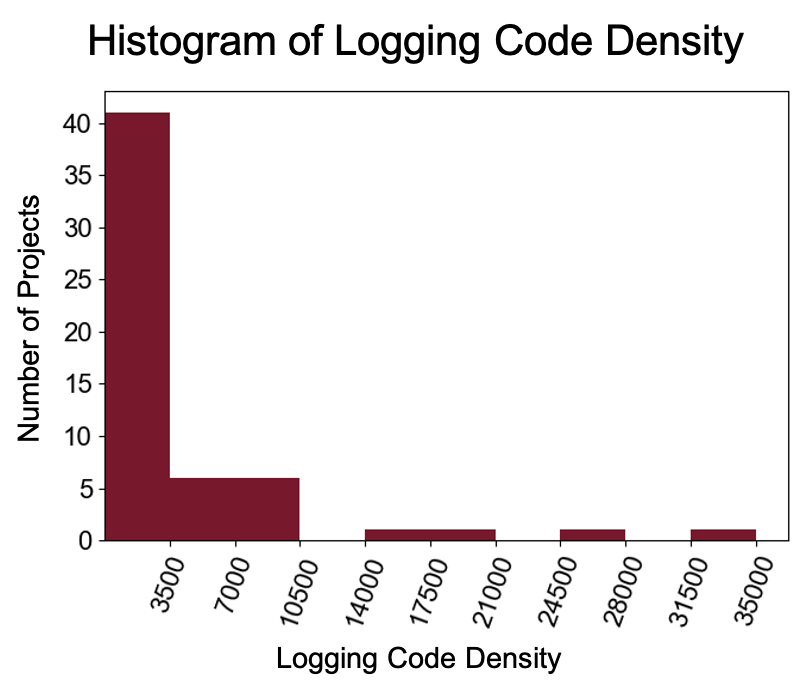
\includegraphics[width=.8\linewidth]{images/mobile-analytics-logging/logging-code-density.png}
  \captionof*{figure}{Density}
  \label{fig:logging-code-density}
\end{minipage}
    \caption{Characteristics of logging}
    \label{fig:logging_rq_1}
\end{figure}

\begin{figure}
    \centering
    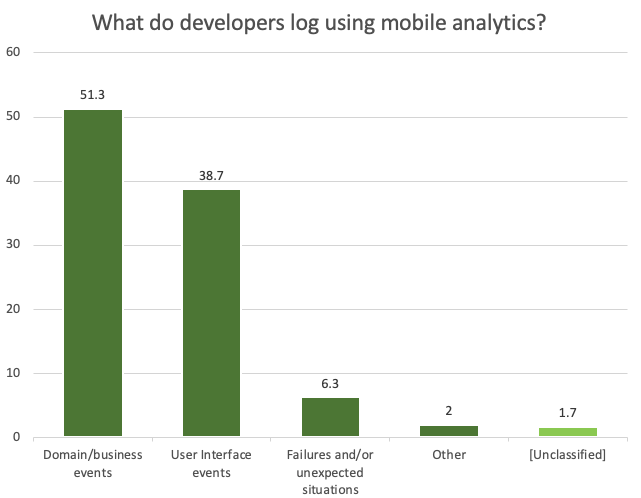
\includegraphics[width=15cm]{images/mobile-analytics-logging/graph-for-research-question-2.png}
    \caption{What is being logged}
    \label{fig:logging_rq_2}
\end{figure}


\begin{listing}
\begin{minted}[
    gobble=4,
    frame=single,
    fontsize=\tiny,
    breaklines=true
  ]{kotlin}
      private fun configureLogging() {
        if (BuildConfig.DEBUG) Timber.plant(Timber.DebugTree())
    }
\end{minted}
\caption{Source~\href{https://github.com/duckduckgo/Android/blob/2f3d42be6a972551c2330daccba6ff4039e1c1a8/app/src/main/java/com/duckduckgo/app/global/DuckDuckGoApplication.kt\#L177-L179}{Lines 177-179 of DuckDuckGoApplication.kt}}
\label{listing:duckduckgo_timber_debug_logging}
\end{listing}

The short source code snippet in Listing~\ref{listing:duckduckgo_timber_debug_logging} provides an example of how developers can choose to vary, or control, the behaviour of the logging for particular builds of their app.


\subsubsection{SmartNavi}
I followed up with one of the 57 projects, the \href{https://smartnavi.app/home}{smartnavi app}~\footnote{The follow-up was triggered by me noticing some problems with a Google website that redirected to an old URL for the project which was now used for insalubrious content. I chose to alert both Google and the project owner so they could address any issues.}.


\textit{The following raw notes are from one of my email updates, on \nth{28} July 2020}

I had my call with Christian Henke who created the project. Here are various notes that are pertinent to our joint research into logging.
\begin{itemize}

    \item The project uses crash reporting (to catch, report, and analyse crashes) and mobile analytics (to try to ascertain where users do and don't use the app). In terms of our coding his use mainly focuses on events generated when users interact with his app.
    \item The app is mature (5+ years) and originally had analytics de developed himself using MySQL, etc. to record the events. He did this mainly to learn about the topic, he was a bachelors|masters student at the time.
    \item Over the years he's used Firebase and Google Analytics mainly for tracking the popularity and use of the app's features. One of the key challenges for this app in his estimation is helping users who don't understand GPS, etc. why the app may be relevant to them. It saves battery life because of the ways it tracks movement, and is mainly intended for people moving at walking pace (rather than in high-speed vehicles).
    \item He also uses Firebase tools to perform A/B experiments related to tutorials and their usability and effectiveness.
    \item He spent a lot of time a year or so ago where he actively focused on fixing crashes being reported in Fabric Crashlytics (since superseded by Firebase Crashlytics). The few crashes that remain are ones either too impractical to investigate (e.g. on a few unbranded low-end Android devices he has no access to) or in a third-party library that only occurs again on a few unusual devices.
    \item The app can run in the background and provide GPS services to other apps e.g. to Google Maps. This has some interesting challenges where Android on various devices and in various conditions may suspend some background activities automatically. If analytics could help track how the background activity is working (and when it's no longer running) that might be very helpful to him and enable him to improve the app's behaviours when run in the background.
    \item He's not proactively working on the app currently. He may spend more time on it soon if he perceives there are new users/use cases for the app. Separately to our research I may help find one or two projects that would be motivating for him e.g. related to mapping Tanzania.
    \item He does coach students at his old university in Germany who are studying marketing. They do various practical exercises to help them gain better marketing skills.
\end{itemize}

We've agreed that there's little more to be gained from asking more about his current quiescent use of analytics since he only checks the analytics infrequently in Firebase (he checked it while we were talking, previously it was around 8 weeks ago he thought). He is happy for others to collaborate on the project, to use it, etc.

\subsection{Outcomes} 
\textit{(Describe the outcomes resulting from the intervention); }


\subsection{Discussion} 
\textit{(Explore what these outcomes mean for the use of analytics in mobile software more generally)}

This case study found the developers of these 57 apps used Mobile Analytics sparsely and the relevant source code was long-lived. Furthermore, what developers chose to log using Firebase differed materially from what similar developers chose to log locally in their codebases. The combination of these findings are worth comparing with the various industrial case studies and these comparisons will be covered later in this thesis %MUST_DO and then add cross-reference link here.  

In hindsight, only finding 7 apps use that firebase logging in F-Droid was a paradox. They were paradoxically too few for the research to be material and too many as F-Droid state they do not accept any apps with Firebase or other non-open Analytics SDKs. The inclusion policy of F-Droid effectively excludes any apps that use Firebase (which they list explicitly as a blocker, along with Crashlytics.)~\url{https://f-droid.org/en/docs/Inclusion_Policy/}. The lack of Firebase Analytics in F-Droid is almost the inverse of what commercial developers do in their Android apps, where over 62\% of all apps include Firebase Analytics, and over 90\% of the top applications do.


\begin{itemize}
    \item Threats to validity include: opensource projects not being very representative of commercial apps; our method where we relied on prior work for our comparisons; use of basic regular expressions; use of srcml that doesn't support Kotlin.
    \item It's an open question whether the opensource developers are using Firebase analytics for similar purposes to the purposes identified in our research. This can be cross-correlated with the interview with Jakob D. where they used Firebase Analytics to capture runtime issues. Admittedly a tiny sample of 4 responses replied to Maurício Aniche's request on Twitter~\url{https://twitter.com/mauricioaniche/status/1250687381914750976} %A copy of the tweet and replies is stored in my misc references folder.
    \begin{itemize}
        \item Pedro Pessoa \href{https://twitter.com/pedpess}{@pedpess} Apr 16, 2020 Replying to @mauricioaniche \emph{``Depends... Usually, critical parts of the biz. For instance, if I can order something from the app, I wanna know if the order succeeded or failed and why... For pure native, I was using Firebase - Crashlytics. Lately, for React Native, Sentry."}
        \item Marabesi Personal computerFlag of Brazil \href{https://twitter.com/MatheusMarabesi}{@MatheusMarabesi} Apr 16, 2020 Replying to @mauricioaniche \emph{``Sentry/bugsnag"}
        \item Robson Soares Amorim \href{https://twitter.com/AmorimRob}{@AmorimRob} Apr 16, 2020 Replying to  @mauricioaniche \emph{``Currently, using App Center to track logs from crashs and custom errors messages in try catchs blocks, personalized events (user clicked on button save, for example). Also, the analytics data provided is very useful for viewing new version adoptions, user session time, devices .."}
        \item Roman Sirokov \href{https://twitter.com/RSirokov}{@RSirokov} Apr 16, 2020 Replying to  @mauricioaniche \emph{``@Firebase has a lot of extremely helpful cross-platform tools; starting from detailed crashlytics, going to app’s performance metrics and user analytics. It’s also possible to implement custom events."}
    \end{itemize}
\end{itemize}

Both this case study and the related work may suffer from the Streetlight effect~\citep{wikipedia_streetlight_effect}, where we research where we can based on sources that are easier to obtain.

\subsection*{Further Work related to this case study}
Further work can be summed up as: ask the devs, concurrent analysis of all the forms of logging, understanding context, and better tooling.

\textbf{Ask the developers:} as mentioned earlier, with one exception, we did not discuss the source code with the authors. We had planned to survey the developers and we believe there would still be merit in doing so to obtain their perspective, experiences, and insights into their use of Firebase Analytics.

\textbf{Concurrent analysis of all logging} This research built on closely-related and relatively recent analysis of similar opensource Android projects. This approach enabled the team to accelerate the initial work and identify broad differences between how Android opensource developers used local and mobile analytics logging. However, by not comparing both local and mobile analytics logging in the same codebases at the same time may have led to inaccuracies in the comparisons. Concurrent analysis of all the forms of logging in the same repos at the same time would help to reduce the scope for inaccuracies and may lead to additional insights.

\textbf{Understanding context}

\textbf{Signal strengths} \textit{c.f. ``On the Naturalness and Localness of Software Logs"} MSR 2021

\textbf{Better tooling} There are several alternative approaches to querying GitHub including the pydriller project (described in~\citep{spadini2018_pydriller}), GitHub's GraphQL API~\footnote{\url{https://docs.github.com/en/graphql}}, and others. These may improve the filtering and selection process. There is also another dataset of verified opensource Android apps on GitHub, ~\href{https://androidtimemachine.github.io/}{AndroidTimeMachine}, described in~\citep{geiger2018_a_graph_based_dataset_of_commit_history_of_realworld_android_apps}. This was co-authored by one of the collaborators for this case study. Unlike our work, theirs includes metadata extracted from Google Play Store; details of their matching and data retrieval process are documented online~\url{https://androidtimemachine.github.io/dataset/} and their implementation is also freely available~\url{https://github.com/AndroidTimeMachine/open_source_android_apps}. Their approach could be used to improve our assessment of liveness and validity of the source repositories, and it might also accelerate aspects of the data collection and filtering.

Furthermore there are various code analysis tools including: LGTM~\footnote{\url{https://lgtm.com/help/lgtm/customizing-code-extraction}} which provide ways to query codebases for specific calls, and CodeScene which tracks the history of changes in the codebase. These may provide more streamlined and production-refined approaches to analysing the code. These would augment rather than replace the value of asking the developers for their perspectives and insights into their choices in selecting and using mobile analytics to monitor reliability and additional software qualities. 


%%%%%%%%%%%%%%%%%%%%%%%%%%%%%%%%%%%%%%%%%%%%%%%%%%%%%%%%%%%%%%%%%%%%%%%%
\par\noindent\rule{\textwidth}{0.4pt}
~\textbf{Earlier material follows}

Logging and mobile analytics intersect with each other, particularly in terms of how they are implemented and in using them to record aspects of the runtime behaviour of software. Previous case studies in this thesis focused on the use and application of various forms of mobile analytics, this section focuses on some of the details of the implementation of logging and the use of mobile analytics to provide a form of remote logging. 

Here we cover:
\begin{itemize}
    \item analysis of logging practices via Firebase Analytics in 107 opensource Android apps,
    \item tools and utilities developed to facilitate the capture and testing of logging in Android apps,
    \item followed by a discussion the design and testing of logging pertaining to Android apps.
\end{itemize}

Logging orients to line-item details and analytics to patterns in what has been logged when the data is aggregated.

\subsection{TODO Materials to incorporate}
\textit{This subsection is to remind me of my various sources for this case study. This entire subsection needs removing once I've done so.}
\begin{itemize}
    \item My draft paper on improving logging.
    \item The MOBILESoft 2021 paper, under review currently.
    \item Various notes in `Notes' on my macbook account.
    \item Bits and pieces related to Shonan Meeting 152. The report provides a useful reminder. Note, for my hysteresis concept we can also add the adaption and application of enterprise tools e.g. using ELK stack.  
\end{itemize}

%After covering various aspects of logging in proprietary apps and codebases, this section addresses three topics with a common focus on logging and logging tools available in opensource projects. It covers two aspects, with a subsequent discussion on the design and testing of logging:

As we learn to program we also enjoy seeing the program output things to show it's doing something under our control, when we run the program we see messages being output, when we don't run it, we don't - concomitant variation in action!~\citep{mill1884system}. Listing~\ref{code:basic_example} is a representative example of the sort of program some of us would have written in BASIC, equivalent output statements exist in many programming languages. Examples to say `Hello World' are available in 28 programming languages~\citep{helloworld2017}. 

% https://www.overleaf.com/learn/latex/Code_Highlighting_with_minted
\begin{listing}
\caption{A representative first BASIC program} \label{code:basic_example}
\begin{minted}{basic}
10 cls
20 print "Hello, world!"
30 sleep
40 end
\end{minted}
Source: \href{https://en.wikibooks.org/wiki/BASIC_Programming/Beginning_BASIC/Your_First_Program}{en.wikibooks.org/wiki/BASIC\_Programming/Beginning\_BASIC/Your\_First\_Program}
\end{listing}

Programmers continue to write and use output statements to observe aspects of what a program is doing, the values of variables, and so on. This includes programmers who develop mobile apps. They can use core components in a programming language, such as a \texttt{printf\{'...'\}} statement, logging libraries, such as \texttt{Log.w\{'...'\}} from the core \mintinline{java}|Android.util.Log|
library, custom logging libraries such as timber, and proprietary libraries. They can also use Mobile Analytics libraries for logging purposes which is what led to this case study.
% https://tex.stackexchange.com/questions/45756/inline-code-and-short-verb-with-minted

Mobile platforms include an operating system that runs on the device; both Android and iOS are based on UNIX. UNIX includes three standard terminal I/O devices: \texttt{stdin}, \texttt{stdout}, and \texttt{stderr}. Of interest here are \texttt{stdout} and \texttt{stderr} which are both output devices, that output text and errors respectively. Developers can therefore use these in their programs, albeit the platform providers (Google and Apple) recommend developers use logging libraries instead. These I/O devices can be redirected the log files on the devices as various people note.

\textbf{Android} includes: comparing ways to redirect \texttt{stdout} to logcat [the standard Android log]~\citep{krysmanski2012_so_redirect-stdout-to-logcat-in-android-NDK, rcdailey2018_ndk_redirect_to_logcats}, and an elegant solution for native code is described in~\citep{tsiombikas2014_native_NDK_stdio_to_android_log}.

\textbf{iOS} includes: 

By default the output of programs are local to the computer the program runs on. This characteristic limits the ability for programmers to observe or analyse the outputs, they need to be local and see the logs as they are generated. 
%
When programs run remotely from the developer they cannot see the logs directly. Many tools exist for collecting and analysing logs from servers and systems, conversely few tools exist to obtain logs from end-user device, which include their smartphones and tablets. Nonetheless, runtime logs are still of interest to developers of mobile apps both for local debugging (generally pre-release) and for remote analysis.



\subsection{How do developers of opensource Android apps use Firebase Analytics?}
\begin{enumerate}
    \item Analysis of third-party opensource Android apps that incorporate Firebase Analytics.
    \item Tools we created to facilitate the testing and analysis of logging by Android developers.
    \item Discussion in methods to improve the effectiveness of logging and the analysis of log messages generated by apps.
\end{enumerate}

Logging is an integral part of the software development process, ranging from sometimes seemingly random print statements to using fully featured software libraries and sophisticated software systems to transfer, replicate, store and analyze log data. Logs are also important developer aids for diagnosing problems and errors, with many app developers collect crash logs for their app from end-user devices - some even ask users for permission to send crash logs when problems occur.  This use of logging is particularly important for mobile software development, where developers need to understand the difference between between effects of the runtime environment, such as poor connectivity, from behaviours of the app when handling the various runtime conditions.

When developers incorporate mobile analytics in their apps, what do they use them for? 

In earlier case studies in this thesis several commercial developers shared their practices informally. This case study complements their insights by analysing 107 opensource Android projects that use Google's Firebase Analytics (the most popular and prevalent in-app analytics tool) to answer two research questions:
\begin{enumerate}
    \item What are the characteristics of logging practices with mobile analytics?
    \item What do developers log with mobile analytics?
\end{enumerate}

This research was performed jointly with an international group of researchers, all-bar-one, met at the~\textit{\nth{152 }NII Shonan meeting~\citep{nii_shonan_workshop_152}} where a group of us agreed to investigate the use of logging in mobile applications as a follow-up activity. We wrote and submitted our first paper in October 2020 where I am the first author. The paper is currently under review. The materials are available as an opensource project at \url{https://github.com/mobileanalyticslogs/mobileanalyticslogging/}.



Early research explored ways developers of opensource Android apps use local logging, a complementary and oft used approach intended to help developers learn more about how their app behaves locally at run-time. MUST-DO provide context either here or in the related works chapter.



MUST-DO continue to write up our post-shonan paper.



\subsubsection{Tacit/default use of analytics}
50 of the 107 codebases studied ... expand with contents from the collaborative research post Shonan. Cross-link my material on tacit logging here.

\subsection{Tools to facilitate capture and testing of logging}

\begin{itemize}
    \item \href{https://github.com/ISNIT0/log-searcher}{\textbf{Log Searcher}}:
    \item \href{https://github.com/ISNIT0/logcat-filter}{\textbf{Logcat Filter}}:
    \item \href{https://github.com/ISNIT0/log-complexity-comparison}{\textbf{Log Complexity Comparison}}:
    \item \href{https://github.com/ISNIT0/AndroidLogAssert}{\textbf{Android Log Assert}}:
    \item \href{https://github.com/ISNIT0/AndroidCrashDummy}{\textbf{Android Crash Dummy}}:
\end{itemize}



\subsection{Discussion on practical aspects for the design, incorporation, and testing of logging} \label{apx:practical-aspects-for-design-and-incorporation-of-logging}
%This appendix introduces various practical aspects of incorporation of mobile analytics that are not necessary to understand the overall approach. The intention is to help those who would be actively involved in the concepts and approach described in the core thesis.
This introduces germane aspects of the design and incorporation of logging...



\subsection{Designing logging}
Unstructured logging can serve immediate needs, for instance to trace code execution or display the value of a variable at run-time. The resulting entries into a log file have limited value in terms of longer term analysis and they may also be harder to identify, filter, and lack relevant content for such analysis.

In the domain of logging both business and research consider logging design important and valuable. 

Storage and transmission of log entries. Sematext provides opensource libraries for Android~\citep{github2020_sematext_logsene_android} and iOS.

Controllable logging: Developers can optionally provide facilities to control the amount of logging that is performed by the app. The well-established K-9 Mail Android app includes optional debug logging that users can activate to help developers diagnose problems and errors~\citep{github2020_k9mail_logging_errors}. A good example of this feature being used is issue 2705 \emph{``Deleted mail from inbox is doubled in trash directory"} on their GitHub site where various users contributed logs and additional information~\citep{github2017_k9mail_issue_2705}. Out of interest, the issue took 20 months to address and multiple contributions before the development team determined the cause, according to the updates in the issue. The project team uses this facility extensively; by \nth{23} December 2020 they had 11 open and 128 closed issues that included the keyword~\href{https://github.com/k9mail/k-9/issues?utf8=\%E2\%9C\%93\&q=is\%3Aissue\%20is\%3Aopen\%20loggingerrors\%20}{loggingerrors}.
% Note: in 2017 the project has 30 open issues and 39 closed, which reference the LoggingErrors wiki page. https://github.com/k9mail/k-9/issues?utf8=%E2%9C%93&q=is%3Aissue%20is%3Aopen%20loggingerrors%20 Some issues are waiting for logging to be provided, others include the requested logcat output.

Materials to incorporate on designing logging:
\begin{itemize}
    \item Retrace from Stackify: Logging meets monitoring. Full lifecycle APM.~\url{https://stackify.com/}
    \begin{itemize}
        \item \url{https://docs.stackify.com/docs/error-and-logs} Logging Rate, Top Errors, Recent Errors, Top Error Chart, Error Rates in dev, test and production.
        \item Application Performance: Slow Pages, Performance Breakdown, Slow Query, Server Performance, Satisfaction Breakdown.~\url{https://docs.stackify.com/docs/application-performance-widgets}
        \item Monitoring and Metrics, App Score:~\href{https://docs.stackify.com/docs/app-score-widgets}{https:// docs.stackify.com/docs/app-score-widgets}.
        \item Centralized Logging: 
        \item Filters, Fields and Tags, and Querying logs:~\url{https://docs.stackify.com/docs/logs-dashboard}. Monitoring logs. 
    \end{itemize}Control Which Logs are Sent to Stackify; ~\texttt{Enrich.WithProperty};~\texttt{stackifyLogger.ForContext}~\url{https://docs.stackify.com/docs/errors-and-logs-serilog}. \emph{``Our .NET libraries automatically handle batching, compressing, queuing, throttling, and error retry logic for uploading your application logs."}\url{https://docs.stackify.com/docs/errors-and-logs-net-supported-frameworks}. \url{https://docs.stackify.com/docs/troubleshoot-errors-and-logs-net-configurations} 4 steps to troubleshooting logging to Stackify's systems. And possibly use the App Score somewhere else in the thesis?~\url{https://docs.stackify.com/docs/appscore}
\end{itemize}

Implementation choices: 

\subsection{Testing logging}
Unit testing of logging to date has not been widely available as a core capability of the logging libraries. There are several possible approaches to asserting the logging is as expected, these include recording the log output \emph{within} the software \emph{i.e.} in memory, and checking what has been written to an actual log [file]. The first approach is described in \citep{altindag2020_unit_testing_log_messages_made_easy} and made available as an opensource project called LogCaptor~\citep{log-captor-github-project}. The second approach was implemented jointly by myself and Joseph Reeve and made available as an opensource project~\citep{android_log_assert}. Both these approaches assert that what was intended to be in the log actually appears there. At the time of writing, the LogCaptor includes richer examples. Our work supports the standard Android logging API in addition to custom logging libraries. As both projects are opensourced and have permissive licenses there is the opportunity to improve either or both of them and for cross-fertilisation.

